%!TEX root = index.tex
\chapter[Revisão Bibliográfica]{Revisão Bibliográfica}
\label{chap:revisao}
\section{Parceria Universidade-Empresa}
\label{cha:ensino}
\subsection{A universidade empreendedora}
\label{cha:univ_empreend}

Ao longo da história as universidades sofreram alterações no seu papel diante da visão da sociedade, mudando grande parte de suas características e atividades. Segundo \citeonline{etzkowitz2001}, duas revoluções aconteceram no modelo de funcionamento da universidade.

Como instituições de origem medieval, as universidades tinham como principal objetivo a conservação, preservação e transmissão de sua cultura através das gerações. Conforme o passar dos anos e novas descobertas sendo feitas, surgiram os seminários como principal forma de disseminação de conhecimento, até evoluirem para os modelos de ensino similares aos atuais. Caracteriza-se essa fase anterior às revoluções como centrada no ensino.

A primeira revolução acadêmica ocorre com a evolução dos modelos de ensino e universidades adotando um modelo intenso de pesquisa, com a intenção de promover avanços na ciência. Com a transmissão mais acessível de pequenas novas descobertas, as pesquisas começaram a se basear em outras pesquisas já realizadas, gerando um ambiente de pesquisa colaborativa.  Durante e após a Segunda Guerra Mundial nos Estados Unidos, a estrutura de pesquisas começou a receber grandes aportes financeiros, e a equipe de pesquisas começou a crescer de tal forma que foram surgindo necessidades de responsabilidades além das exercidas por alunos e pesquisadores, principalmente em relação à administração dessa estrutura de pesquisas, como manutenção da propriedade intelectual e divulgação de novas descobertas. O ambiente de pesquisas começou a ficar similar a uma empresa, o que levou a segunda revolução da academia.

Com uma estrutura voltada a acelerar o desenvolvimento de pesquisas, os laboratórios passaram a ser vistos como fonte de resolução de problemas reais do mercado. A segunda revolução acadêmica aconteceu quando as universidades passaram a utilizar seus laboratórios de pesquisa para realizar descobertas que pudessem gerar produtos comerciáveis. Desta forma, também foi inserido o desenvolvimento econômico como uma nova missão da universidade, além da pesquisa e do ensino.

\begin{figure}
\caption{Revoluções Acadêmicas}
\centerline{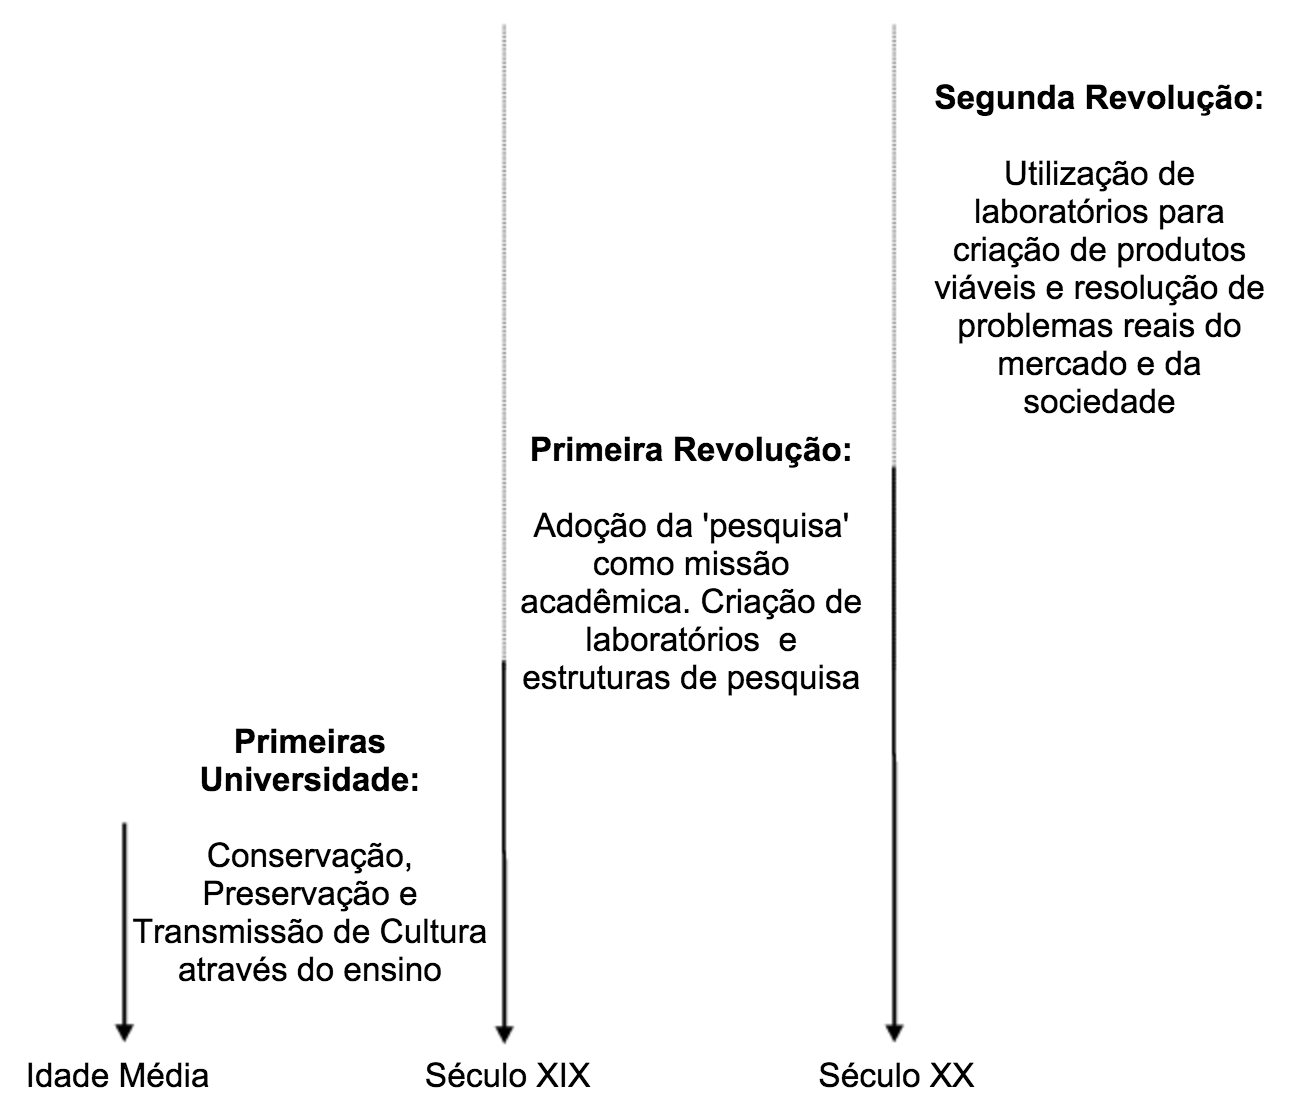
\includegraphics[scale=0.5]{img/academic_revolutions}}
\label{fig:academic_revolutions}
\caption* {Fonte: Elaborado pelo autor a partir de \citeonline{etzkowitz2001}}
\end{figure}

Com o sistema de financiamento de pesquisa da Universidade em  busca de estabilidade, em muitos casos cabe à própria Universidade procurar por novas fontes de receita, gerando novas parcerias com empresas dispostas a investir seu dinheiro em pesquisas.

Dessa forma, surge o conceito de Universidade Empreendedora, que recebe diferentes concepções de diversos autores. Segundo \citeonline{etzkowitz2001}, é uma instituição que trabalha ativamente na transferência de tecnologia e no desenvolvimento econômico, já para \citeonline{burton} é uma instituição que realiza um esforço contínuo de reformulação institucional de forma a melhorar o desempenho para com empresas e o governo, e para \citeonline{plonsky} é uma instituição que exerce um papel ativo no mercado do conhecimento.

\subsection{Interação universidade-empresa-governo}
\label{cha:univ_empreend}

\citeonline{etzkowitz2000} propõe que os modelos de interação entre universidade e empresa refletem na interferência de um terceiro agente, o Governo - ou Estado. Em regimes com forte influência do Estado, como na ex-União Soviética e países do Leste Europeu, o governo regula e direciona as relações entre as empresas e a academia. \ref{fig:triplehelix1}. Esse modelo é visto como um modelo de desenvolvimento falho, pois inibe iniciativas de inovação a partir da empresa e academia, cabendo apenas ao Estado direcionar os estudos a serem realizados.

\begin{figure}[H]
\caption{Modelo de interação universidade-indústria-governo regulado pelo governo}
\centerline{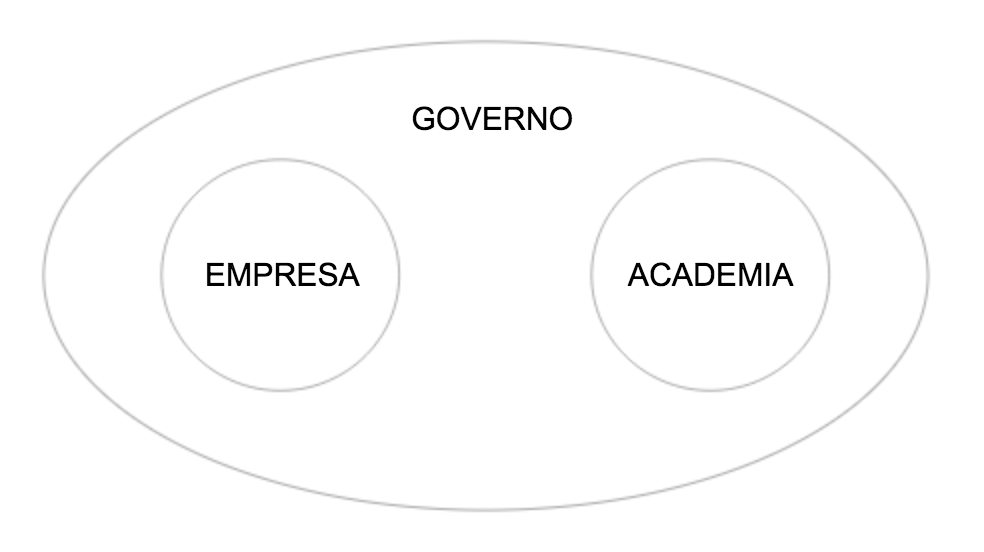
\includegraphics[scale=0.5]{img/triplehelix1}}
\label{fig:triplehelix1}
\caption* {Fonte: Adaptado de \citeonline{etzkowitz2000}}
\end{figure}

Um segundo modelo, apropriado da expressão \textit{laissez-faire}, consiste na minimização da interferência de atuação entre as esferas, principalmente em relação ao Governo, que apresentava total controle no primeiro modelo. Nesse modelo, \ref{fig:triplehelix2}, cada ator atua de forma independente, apenas havendo transmissão de informação entre eles mas não uma colaboração ativa em prol da inovação.

\begin{figure}[H]
\caption{Modelo \textit{laissez faire}, de independência entre universidade, indústria e governo}
\centerline{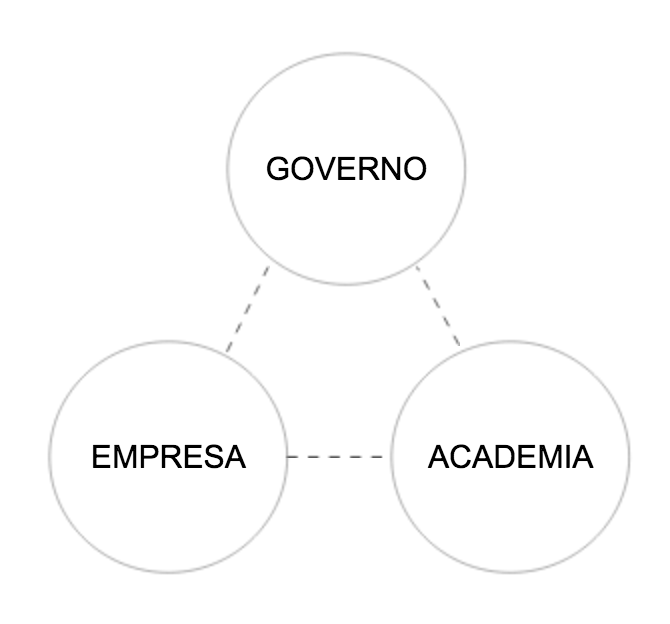
\includegraphics[scale=0.5]{img/triplehelix2}}
\label{fig:triplehelix2}
\caption* {Fonte: Adaptado de \citeonline{etzkowitz2000}}
\end{figure}

Já o terceiro modelo em questão representa de fato a Tripla Hélica Universidade-Indústria-Governo, com uma infraestrutura de conhecimento compartilhada entre as esferas, com funções surgindo através da colaboração, cogestão e compartilhamento de recursos entre os atores, através de organizações emergindo nessas interfaces.


\begin{figure}[H]
\caption{Modelo Tripla Hélice Universidade-Empresa-Governo}
\centerline{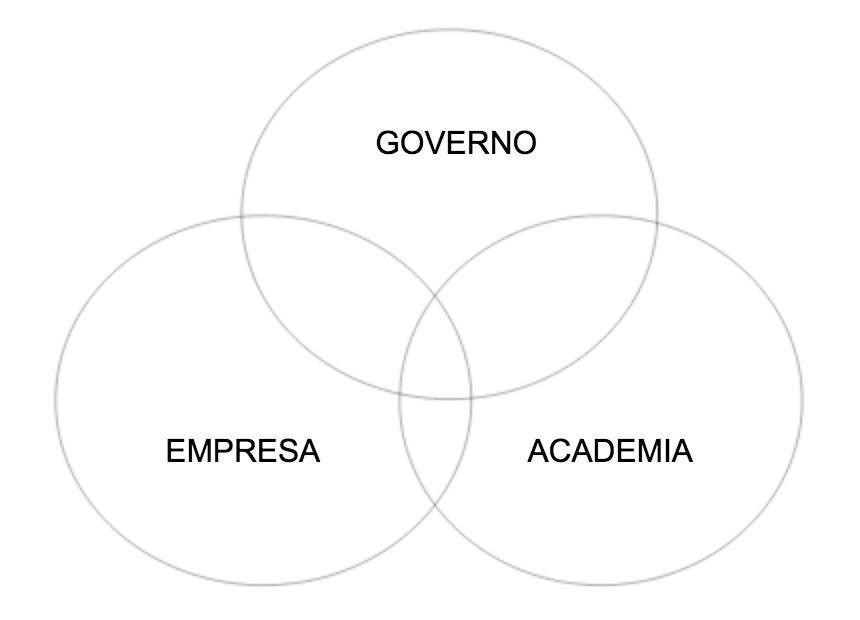
\includegraphics[scale=0.5]{img/triplehelix3}}
\label{fig:triplehelix3}
\caption* {Fonte: Adaptado de \citeonline{etzkowitz2000}}
\end{figure}

No modelo de tripla hélice o Governo assume uma posição de facilitador da interação entre empresa e academia sem tirar a autonomia de ambos os atores. Através de leis de incentivo e financiamento o governo fornece e capta recursos para o desenvolvimento de novas pesquisas, e através da criação de laboratórios e parques tecnológicos oferece uma infraestrutura para  auxiliar no processo de inovação.

\subsection{Desafios da gestão universidade-empresa}
\label{cha:univ_empreend}

\citeonline{plonsky} ressalta a mudança de ênfase da discussão sobre a cooperação entre academia e setor produtivo na época, pois a temática principal deixou de ser ideológica, e sim em relação a gestão dessa parceria. De forma a elucidar essa questão ele define alguns principais desafios gerenciais entre universidade e empresa para manter a relação entre ambos "benéfica e transformadora":

\begin{itemize}
\item Compartilhar uma visão multidimensional e integrada da cooperação universidade-empresa, centrada no desenvolvimento de competências humanas
\item Perceber com clareza as missões distintas, mas complementares, da empresa e da universidade no processo de inovação
\item Desenvolver respostas inovativas às diversas necessidades de cooperação empresa-universidade
\item Capacitar para a gestão eficaz da cooperação empresa-universidade
\end{itemize}

Primeiramente, ambos os lados devem entender que a parceria entre academia e empresa não se limita a projetos específicos e pontuais envolvendo ambas as partes, pois na realidade a parceria se extende a um dos principais objetivos da universidade, que é o de desenvolver alunos para atuar no mercado de trabalho. De forma geral, o setor produtivo deve estar sempre estar interessado na qualidade e na atualização do ensino das universidades pois consequentemente serão formadas pessoas mais capacitadas.

Em seguida, deve ficar evidente que empresa e universidade possuem papéis distintos no processo de inovação. A universidade assume na inovação o papel de organizar todo o conhecimento em relação a determinados assuntos. Já o desenvolvimento de tecnologia corresponde à aplicação do conhecimento organizado na produção de bens e serviços e, de forma geral, é de responsabilidade da empresa.

Embora existam diferentes necessidades de ambas as partes advindas da parceria universidade-empresa, deve-se compreender que por mais que a relação seja assimétrica, uma verdadeira cooperação não só deve ser benéfica como também deve gerar aprendizado para ambas as partes. Logo as respostas inovativas devem surgir mais rapidamente com ambos os lados sendo capacitados e beneficiados.

Por fim, todo caso de cooperação empresa-universidade deve estar sob gestão de um \textit{staff} pré-capacitado, pois uma série de conhecimentos acabam sendo necessários para tirar o máximo de proveito dessa parceria, como: desdobramento de missão e visão institucional; proteção de propriedade intelectual; equacionamento econômico-financeiro, gestão de projetos, entre outros.

\section{Metodologia de Entrevistas}
\label{cha:ensino}
